\documentclass[border=0.2cm]{standalone}
\title{GSA Analysis Iteration Procedure}
\author{Jianer Cong}
\usepackage{tikz}
\usepackage{minted}
\usemintedstyle{vs}
\setminted{bgcolor=gray!30}             %all lang has ling numbers

% Use Cascadia code for texttt
\usepackage{fontspec}
\setmonofont{Cascadia}[
Path=/usr/share/fonts/truetype/Cascadia_Code/,
Scale=0.85,
Extension = .ttf,
UprightFont=*Code,              %find CascadiaCode.ttf
BoldFont=*CodePL,               %find CascadiaCodePL.ttf ...
ItalicFont=*CodeItalic,
BoldItalicFont=*CodePLItalic
]

% tikz libraries
\usetikzlibrary{shapes} % ellipse node shape
\usetikzlibrary{shapes.multipart} % for line breaks in node text
\usetikzlibrary{arrows.meta}    %-o arrow head
\usetikzlibrary{arrows}
\begin{document}
\documentclass[border=0.2cm,dvipsnames]{standalone}

\newcommand{\mycola}{Blue}
\newcommand{\mycolb}{Sepia}
\newcommand{\mycolc}{OliveGreen}

\newcommand{\cla}[1]{\textcolor{\mycola}{#1}}
\newcommand{\clb}[1]{\textcolor{\mycolb}{#1}}
\newcommand{\clc}[1]{\textcolor{\mycolc}{#1}}
\title{p}
\author{Jianer Cong}
\usepackage{tikz}
\usepackage{tcolorbox}
\usetikzlibrary{shapes} % ellipse node shape
\usetikzlibrary{shapes.multipart} % for line breaks in node text
\usetikzlibrary{arrows.meta}    %-o arrow head
\usetikzlibrary{arrows}

\begin{document}
% 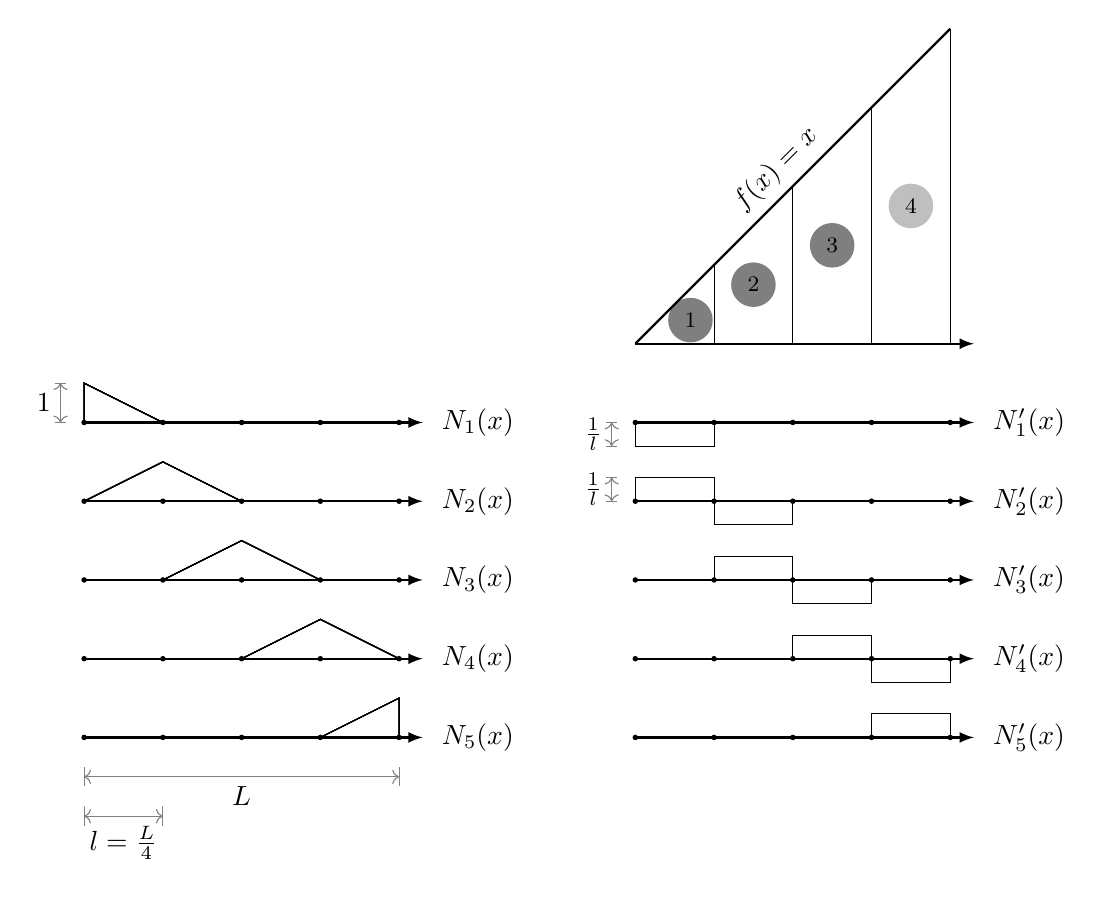
\begin{tikzpicture}[x=1cm,y=1cm]
  \begin{scope}
    % \draw[style=help lines,step=1cm] (0,-1) grid (11,5);

    \foreach \y in {0,1,2,3,4}{%
      \foreach \x in {0,7}{%
        \draw[-latex,thick] (\x,\y) -- +(4.3,0);
        \foreach \z in {0,1,2,3,4}{
          \fill[black] (\x + \z, \y) circle (1pt);
        }
      }



      \newcommand{\myh}{0.5}
      \draw (0,4) -- ++(0,\myh) -- ++(1,-\myh);
      \draw (3,0) -- ++(1,\myh) -- ++(0,-\myh);
      \foreach \i in {0,1,2}{
        \draw (\i, 3 - \i) -- ++(1,\myh) -- ++(1,-\myh);
      }
    }

    \foreach \i in {0,1,2,3}{
      \foreach \j in {0,0.7}{
        \draw (7 + \i, 3 - \i + \j) rectangle +(1,0.3);
      }
    }
    \foreach \y in {1,2,3,4,5}{
      % Label each diagram
      \node at (5, 5 - \y) {$N_{\y}(x)$};
      \node at (5 + 7, 5 - \y) {$N_{\y}'(x)$};
    }

  \end{scope}

  \newdimen\h
  \h=3.5pt

  % Draw the two dimensions
  \begin{scope}[draw=black!50]
    \foreach \i / \j / \l in {0.5 / 4 / L, 1 / 1 / l=\frac{L}{4}}{
      \draw[thin,<->] (0,-\i) to node[anchor=north] {$\l$} +(\j,0);
      \draw (0,-\i) -- +(0,\h) -- +(0, -\h)
      (\j,-\i) -- +(0,\h) -- +(0, -\h);
    }

    \h=2pt
    \newcommand{\mydimy}[4]{%
      \draw[thin,<->] (#1,#2) to node[left] {#4} +(0,#3);
      \draw (#1,#2) -- +(-\h,0) -- +(\h,0)
      (#1,#2 + #3) --  +(-\h,0) -- +(\h,0);
    }
    % \draw[thin,<->] (-0.3,4) to node[left] {1} +(0,0.5);
    % \draw (-0.3,4) -- +(-\h,0) -- +(\h,0)
    % (-0.3,4 + 0.5) --  +(-\h,0) -- +(\h,0);
    \mydimy{-0.3}{4}{0.5}{1}
    \mydimy{7-0.3}{3}{0.3}{$\frac{1}{l}$}
    \mydimy{7-0.3}{3.7}{0.3}{$\frac{1}{l}$}
  \end{scope}

  \begin{scope}[xshift=7cm,yshift=5cm]
    \draw[-latex,thick] (0,0) -- +(4.3,0);
    \draw[thick] (0,0) to node[sloped,above]{$f(x)=x$} (4,4);
    \foreach \x in {1,2,3,4}{
      \draw (\x,0) -- (\x,\x);
    }

    \newcommand{\mynode}[3][(0,0)]{
      \node[shape=circle, fill=#3,
      fill opacity=0.5,text opacity=1,font=\footnotesize, shift={#1}] {#2};
      % \node[shape=circle, fill=gray,
      % fill opacity=0.5,text opacity=1,font=\footnotesize, shift={(1cm,1cm)}] {2};
    }
    % \foreach \i/\j/\c in {0.5/1/\mycola,1.3/2/\mycolb,2.3/3/\mycolc,3.3/4/gray}{
    %   \mynode[(\i + 0.2, \i -0.2)]{\j}{\c}
    % }
    \mynode[(0.7, 0.3)]{1}{\mycola}
    \mynode[(1.5,0.75)]{2}{\mycolb}
    \mynode[(2.5,1.25)]{3}{\mycolc}
    \mynode[(3.5,1.75)]{4}{gray}
    % \mynode[(0.5 + 0.2, 0.5 -0.2)]{2}{\mycolb}
    % \mynode[(0.5 + 0.2, 0.5 -0.2)]{3}{\mycolc}
  \end{scope}

\end{tikzpicture}
% \newtcbox{bLabBox}[1][red]{
  on line,arc=0pt,colback=#1!10!white,
  colframe=#1!50!black,
  boxsep=0pt,left=1pt,right=1pt,top=2pt,
  bottom=2pt,boxrule=0pt,bottomrule=1pt,toprule=1pt
}
\newtcbox{nLabBox}[1][red]{
  on line,top=2pt,bottom=2pt,
  left=3pt,right=3pt,
  colframe=#1,
  colback=#1!10!white
}
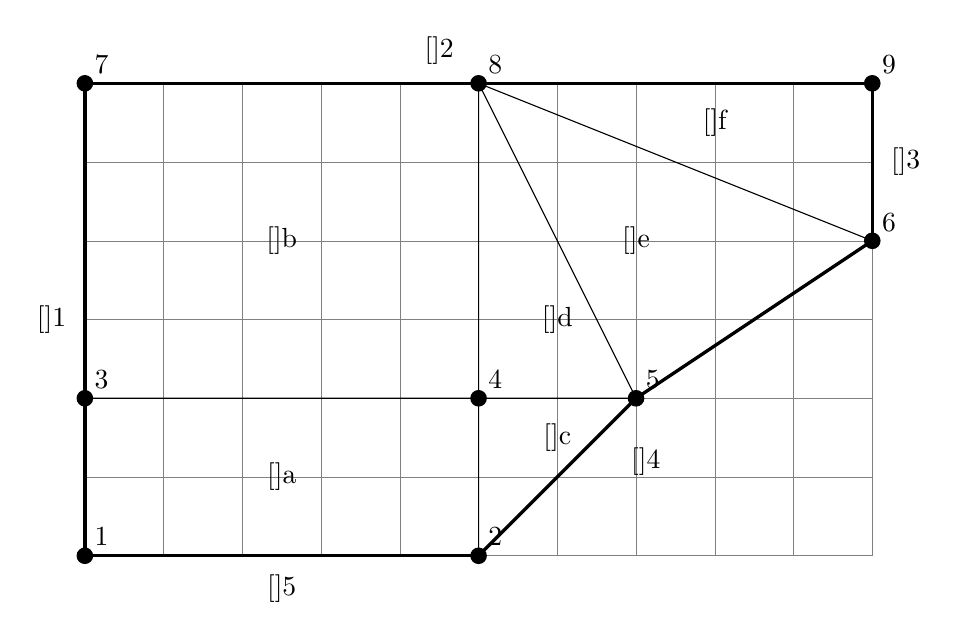
\begin{tikzpicture}[x=1cm,y=1cm]
  \newcommand{\bLab}[4][(0,0)]{
    % \node[fill=#2,text=white,#3] at #1 {#4};
    \node[#3] at #1 {
      \bLabBox[#2]{#4}
    };
  }

  \begin{scope}[very thick]
    \draw[style=help lines,step=1cm] (0,0) grid (10,6);
    % \tikzstyle{every node}=[draw,circle]

    \draw[draw=\mycola] (0,0) -- (0,6);
    \bLab[(0-0.1,3)]{\mycola}{left}{1}

    \draw[draw=\mycolb] (0,6) -- (10,6);
    \bLab[(4.5,6.1)]{\mycolb}{above}{2}

    \draw[draw=\mycolc] (10,6) -- (10,4);
    \bLab[(10.1,5)]{\mycolc}{right}{3}

    \draw[draw=\mycola] (10,4) -- (7,2) -- (5,0);
    \bLab[(7-0.2,1.2)]{\mycola}{right}{4}

    \draw[draw=\mycolb] (5,0) -- (0,0);
    \bLab[(2.5,-0.1)]{\mycolb}{below}{5}
  \end{scope}

  \begin{scope}
    % draw the mesh
    \draw (0,2) -- +(7,0)
    (5,0) -- ++(0,6)
     -- +(2,-4)
     -- +(5,-2)
     -- +(0,0);

     \foreach \x/\y/\l in {
       0/0/1,5/0/2,0/2/3,5/2/4,
       7/2/5,10/4/6,0/6/7,5/6/8,
       10/6/9}{
       \fill[black] (\x,\y) circle (3pt);
       \node[above right] at (\x,\y) {\l};
     }

     \newcommand{\nLab}[3][(0,0)]{
       % \node[fill=#2,text=white,rectangle] at #1 {#3};
       \node at #1 {\nLabBox[#2]{#3}};
     }

     \foreach \x/\y/\l/\c in {
       2.5/1/a/\mycola,2.5/4/b/\mycolb,
       6/1.5/c/\mycolc,6/3/d/\mycola,
       7/4/e/\mycolb,8/5.5/f/\mycolc
     }{\nLab[(\x,\y)]{\c}{\l}}
  \end{scope}
\end{tikzpicture}
% 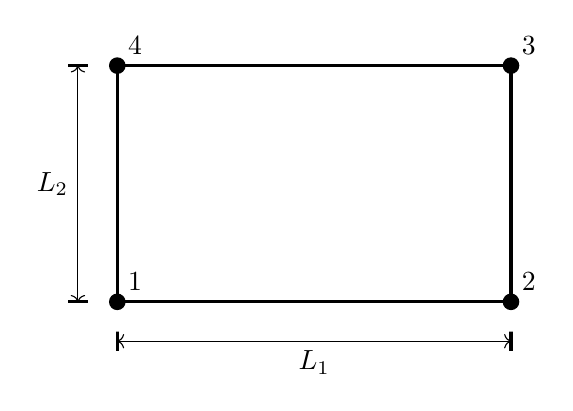
\begin{tikzpicture}[x=1cm,y=1cm]
  \begin{scope}[very thick]
    \draw (0,0) node[above right] (n1) {1}
    --  +(5,0) node[above right] (n2) {2}
    -- +(5,3) node[above right] (n3) {3}
    -- +(0,3) node[above right] (n4) {4}
    -- cycle;

    \foreach \i in {1,2,3,4}{
      % \node[fill=#2,]
      \fill[black] (n\i.south west) circle (3pt);
    }

    \newdimen\h
    \h=3.5pt
    % Draw the two dimensions
    \def\i{0.5cm}
    \def\j{5cm}

    \draw[thin,<->] (0,-\i) to node[anchor=north] {$L_1$} +(\j,0);
    \draw (0,-\i) -- +(0,\h) -- +(0, -\h)
    (\j,-\i) -- +(0,\h) -- +(0, -\h);

    % y dimensions
    \newcommand{\mydimy}[4]{%
      \draw[thin,<->] (#1,#2) to node[left] {#4} +(0,#3);
      \draw (#1,#2) -- +(-\h,0) -- +(\h,0)
      (#1,#2 + #3) --  +(-\h,0) -- +(\h,0);
    }
    \mydimy{-0.5cm}{0}{3}{$L_{2}$}
  \end{scope}
\end{tikzpicture}
\begin{tikzpicture}[x=1cm,y=1cm]
  \begin{scope}
    \draw (0,0) coordinate (n1)
    --  +(4,-1) coordinate (n2) 
    -- +(3,2) coordinate (n3)
    -- cycle;

    \foreach \i/\p in {1/above left,2/below right,
      3/above left}{
      \node[\p] at (n\i) {$(x_{\i}, y_{\i})$};
      \fill[black] (n\i) circle (3pt);
    }
  \end{scope}
\end{tikzpicture}
\end{document}
\end{document}